%!TEX root = ../article.tex

% Solution
\section{Solution}
\label{sec:solution}

In the present work our main goal is to determine if a cloud-based solution can meet the
requirements of RFID-based smart place applications, as mentioned in Section~\ref{sub:objectives}.
To achieve our goals we will follow two approaches to deploy the smart warehouse application: cloud
and fog. In Section~\ref{sub:sol_smart_warehouse_deployment}, we present alternative architectures
of the smart warehouse deployment.\\

Usually, provisioning the components of a smart place application is an operation that is manually executed and
requires expertise since that the software components must be correctly installed and configured.
Furthermore, every time that a new smart place is deployed these operations must be repeated. With
that in mind, in order to make the deployment of smart places more efficient in Section~\ref{subs:sol_provisioning}
we propose a mechanism that automates the provision of smart places application in the cloud.\\

% Smart Warehouse Deployment
\subsection{Smart Warehouse Deployment}
\label{sub:sol_smart_warehouse_deployment}
In traditional solutions, the application is provisioned in a local infrastructure. Although such
approach guarantees that the low-latency requirements are meet, this solution comes with several
downsides - such as the low scalability, infrastructure and maintenance costs - that can be a
barrier for these applications.\\

Leveraging the infrastructure required to provisioning the smart place applications to the cloud
guarantees that the bottlenecks of traditional solutions are solved. However, we also need to
guarantee that the latency requirements of these applications are fulfilled. The cloud and fog concepts
give us more flexibility to perform the deployment of smart place applications, which allow us to
provisioning the application modules in a more distributed way. The following sections describe
the deployment approaches of smart place applications based in the cloud and fog.\\

% Cloud approach
\subsubsection{Cloud Deployment}
\label{subs:sol_cloud}
The warehouse is composed of smart objects, sensors and readers that capture the events that occurs
in the warehouse. The application middleware is provisioned in the cloud, which virtualizes the computing,
storage and network resources needed to support the application. The smart warehouse can be connected
to the cloud through a physical or wireless connection.\\

% Fog approach
\subsubsection{Fog Deployment}
\label{subs:sol_fog}
As in the cloud-based approach the warehouse is composed of smart objects, sensors and readers.
The proposed approach aims to extend the cloud paradigm to the edge of the network. Unlike the
cloud infrastructure, that usually is provisioned thousands of kilometers from the smart warehouse,
the fog infrastructure usually is provisioned closest to the smart warehouse network.\\

Regarding the application middleware, the application components are distributed across the cloud and
fog. The components responsible for storing the data during a long period of time are provisioned in
the cloud. The components responsible for performing real-time processing of the data generated in the
warehouse, and the components that filter the data that is consumed locally and must be delivered to
the cloud are provisioned in the fog. Both the smart warehouse as the fog can be connected respectively
to the fog and cloud through several types of connection, from a physical connection to a wireless
connection.

% Provisioning
\subsection{Smart Place Provisioning}
\label{subs:sol_provisioning}
In this section we propose a mechanism that automates the provisioning of software for smart place
applications in the cloud. Our solution relies on \acrfull{CM} tools that leverage existing software
stacks. Figure~\ref{fig:provisioning_generic_architecture} presents the architecture for the proposed
mechanism.\\

% Provisioning mechanism conceptual architecture
\begin{figure}[ht!]
  \centering
  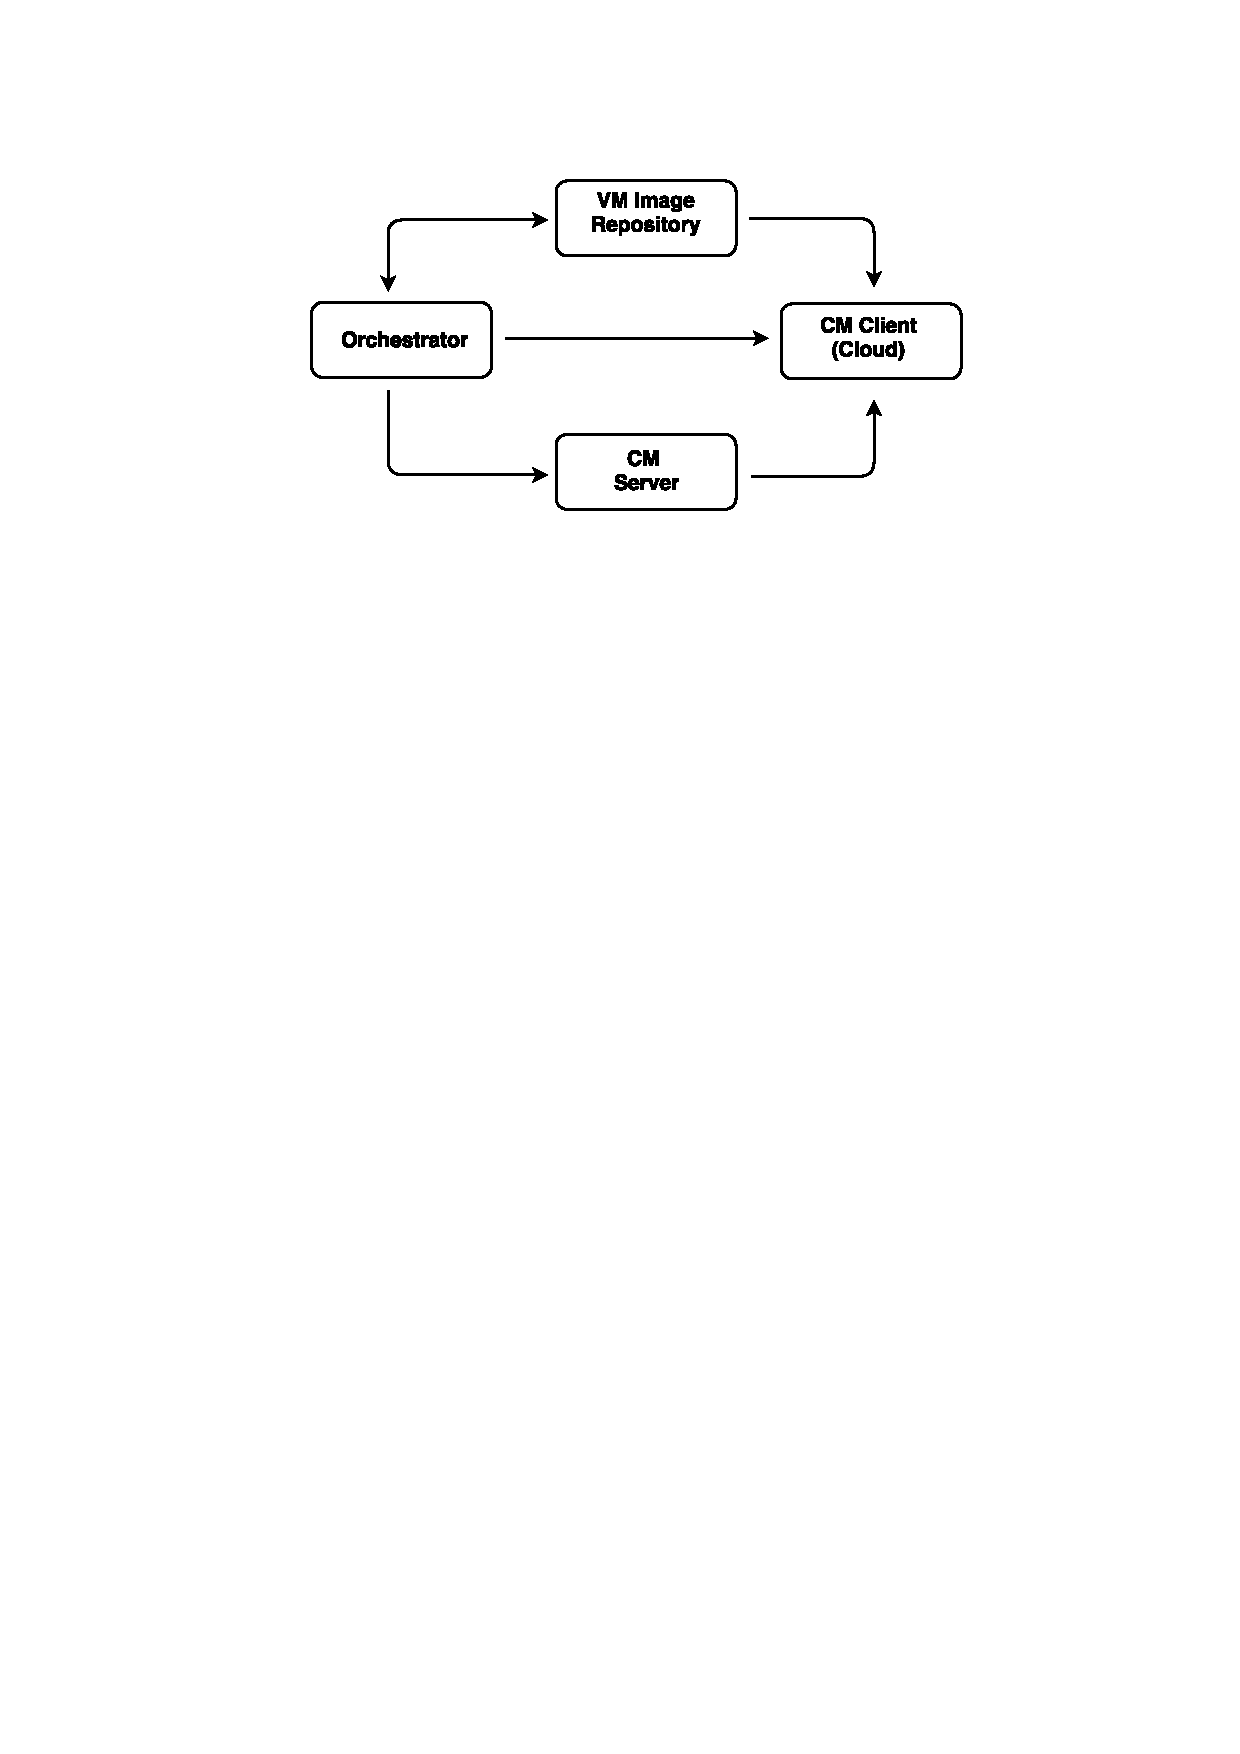
\includegraphics[width=.4\textwidth]{./figures/c4t-generic-solution.pdf}
  \caption[Provisioning mechanism conceptual architecture.]{Provisioning mechanism conceptual architecture.}
  \label{fig:provisioning_generic_architecture}
\end{figure}

In the proposed architecture, the provisioning of a smart place is based on provisioning policies and
software images that are defined and configured in a development environment. The provisioning policies
allow to define which components of software must be provisioned in a given instance, configure
management tasks such as to trigger a notification when a resource state changes. The software images
contains all the software components required to deploy the application.\\

After the provisioning policies were defined and configured, the Orchestrator uploads them to its respective
remote repositories (CM Server and VM Image Repository). When the provisioning request is performed -
through a configuration management interface provided by the Orchestrator - the configuration management
client (\gls{CM} Client) in the cloud server pulls the polices from the configuration management server
(\gls{CM} Server), a centralized server that is responsible to maintain a consistent state of the
provisioned nodes in the cloud. In order to enforce the polices, the \gls{CM} Client pulls the software
images from a central repository and then performs the provisioning and configuration of the software.
After provisioning the infrastructure, the CM client periodically polls the CM server in order to
determine if its current state is consistent with the most recent policy.
